\chapter{Fundamentação teórica}

Este capítulo aborda os conceitos teóricos necessários para a compreensão do presente trabalho.

\section{Aprendizado de Máquina}

O aprendizado de máquina é um subcampo da inteligência artificial que tem por objetivo o desenvolvimento de algoritmos capazes de aprender e tomar decisões a partir de um conjunto de dados, sem que seja necessária a programação explícita para essas tarefas específicas \cite{mlDietterich}. Fundamentalmente, esses sistemas buscam aprender padrões em coleções de dados para, a partir da generalização desse conhecimento, realizar inferências sobre novas informações. Esse processo de aprendizado utiliza modelos matemáticos, principalmente estatísticos, que capturam relações complexas entre variáveis de entrada e saída através do ajuste de parâmetros internos, permitindo que a aplicação melhore seu desempenho conforme é exposta a mais dados \cite{mlSarker,mlDietterich}. Em geral, as técnicas de \textit{machine learning} são categorizadas em três paradigmas principais: aprendizagem supervisionada, não supervisionada e por reforço \cite{mlSarker}.

O aprendizado supervisionado caracteriza-se pela utilização de conjuntos de dados rotulados, onde tanto as entradas quanto as saídas desejadas são conhecidas durante o treinamento. Nesse paradigma, o algoritmo aprende através de exemplos, de forma a possibilitar tarefas como classificação -- a atribuição de classes discretas aos dados, como ilustrado pela Figura \ref{fig:mlsupervised} -- e regressão -- a predição de valores contínuos \cite{mlDietterich}. Algoritmos clássicos dessa categoria incluem máquinas de vetores de suporte, redes neurais artificiais e métodos \textit{ensemble} \cite{mlSarker}.

\begin{figure}[H]
	\caption{\label{fig:mlsupervised}Representação de Aprendizado Supervisionado}
    \begin{center}
    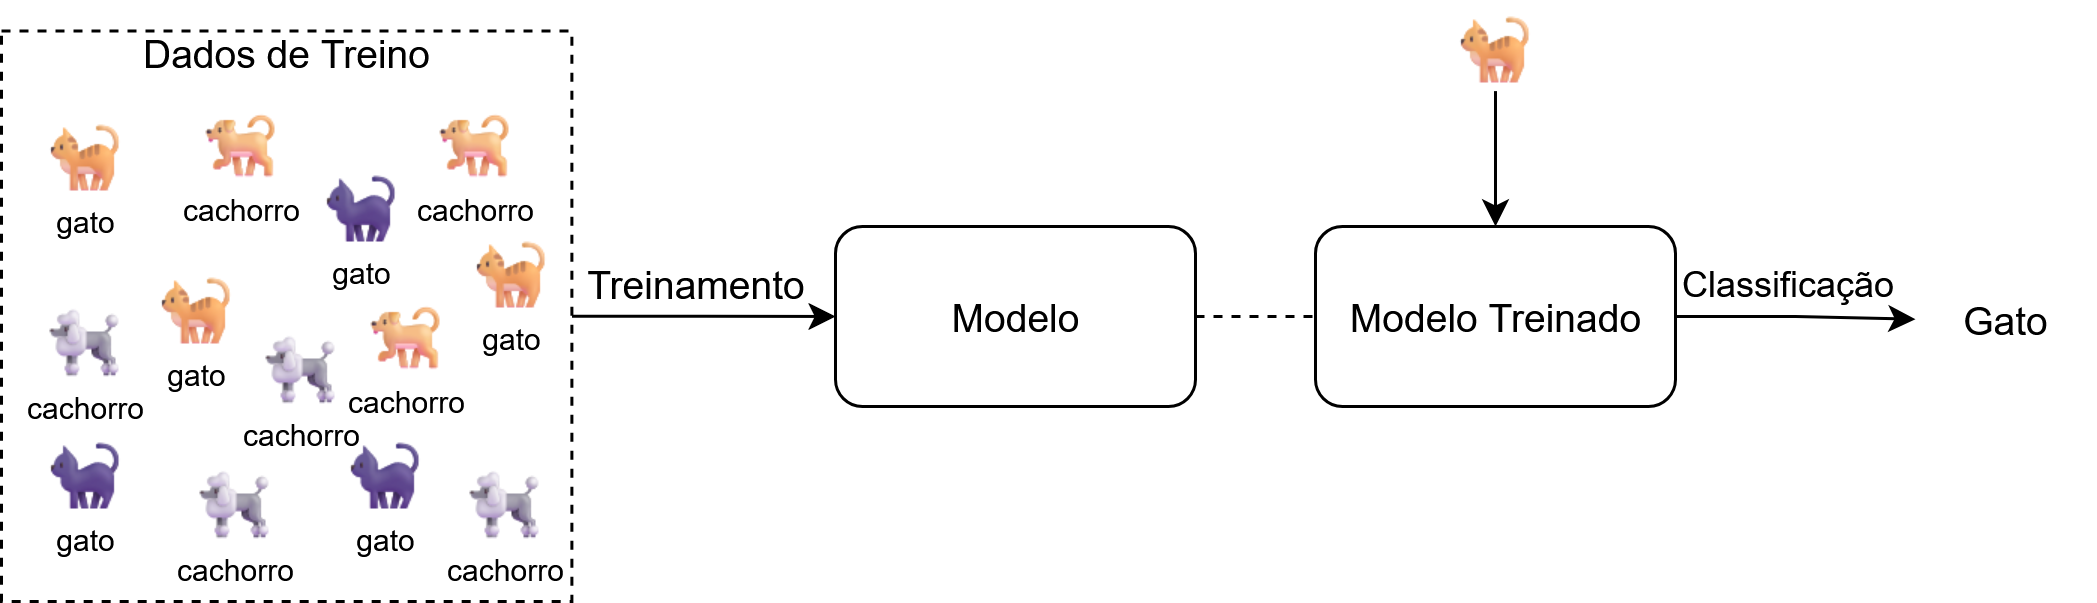
\includegraphics[width=1\linewidth]{images/mlsupervised.png}
	\end{center}
	\fonte{o autor}
\end{figure}

O aprendizado não-supervisionado, por sua vez, opera sobre dados não rotulados, sem o conhecimento das saídas desejadas, e busca compreender a organização natural de um dado conjunto a partir da identificação de padrões intrínsecos. Essa abordagem engloba técnicas como agrupamento (\textit{clustering}), ilustrado pela Figura \ref{fig:mlunsupervised}, e detecção de anomalias \cite{mlSarker}. Ainda, diferentes estratégias de aprendizado podem ser incorporadas, como algoritmos semi-supervisionados, utilizados quando um \textit{dataset} tem poucos dados classificados, de forma a aproveitar a estrutura implícita do conjunto não categorizado para melhorar o desempenho do modelo \cite{mlSarker}.

\begin{figure}[H]
	\caption{\label{fig:mlunsupervised}Representação de Aprendizado Não Supervisionado}
    \begin{center}
    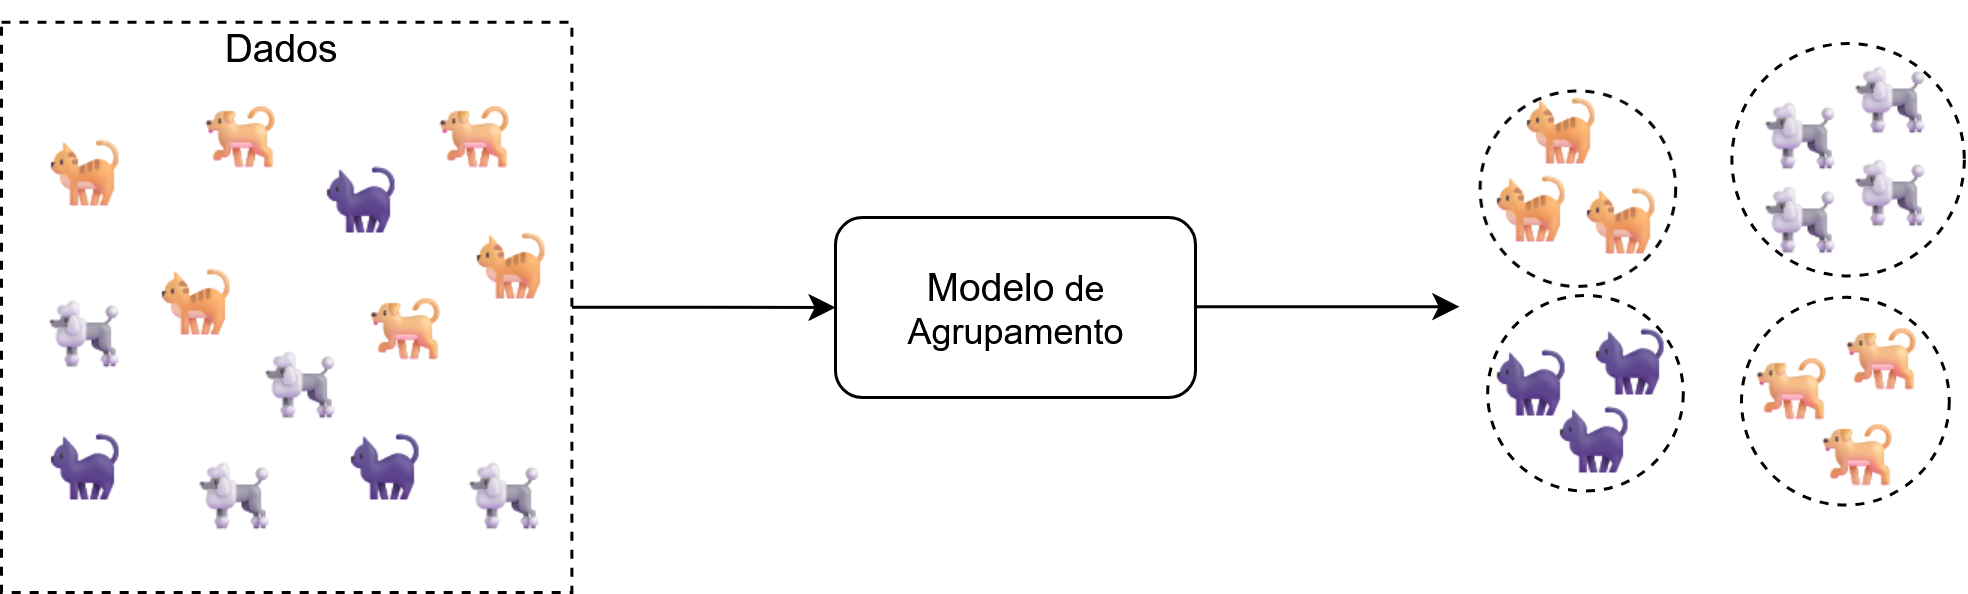
\includegraphics[width=1\linewidth]{images/mlunsupervised.png}
	\end{center}
	\fonte{o autor}
\end{figure}

Adicionalmente, o aprendizado por reforço representa um paradigma distinto onde um modelo aprende através de interações com um ambiente, sendo recompensado ou penalizado com base em suas ações, de forma que gradualmente desenvolva estratégias ótimas \cite{mlSarker}. A Figura \ref{fig:mlreinforced} ilustra o exemplo de um modelo com recompensas positivas para a identificação de cães.

\begin{figure}[H]
	\caption{\label{fig:mlreinforced}Representação de Aprendizado por Reforço}
    \begin{center}
    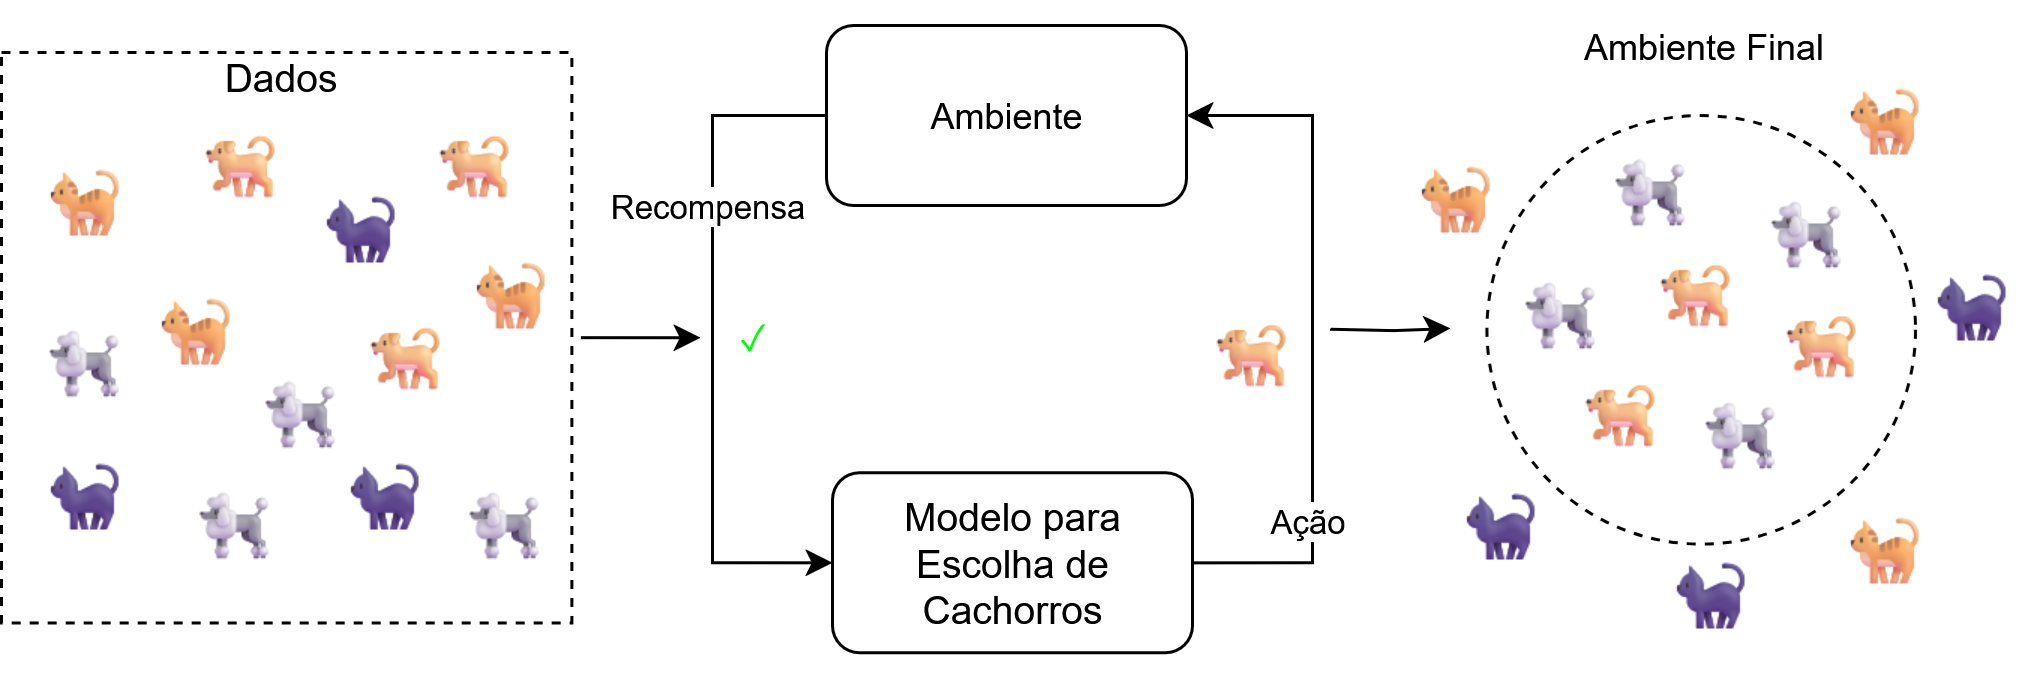
\includegraphics[width=1\linewidth]{images/mlreinforced.png}
	\end{center}
	\fonte{o autor}
\end{figure}

Embora os conceitos fundamentais de aprendizado de máquina tenham sido estabelecidos há quase um século, com contribuições embrionárias nas décadas de 1950 e 1960 \cite{mlDietterich}, essa área de estudo tem recebido grande destaque nas últimas décadas. Esse ressurgimento deve-se principalmente ao aumento exponencial da capacidade computacional e à disponibilidade massiva de dados digitais. Também, a evolução do \textit{hardware} -- particularmente o advento de unidades de processamento gráfico de alto desempenho (GPU) -- possibilitou o treinamento de modelos complexos, antes computacionalmente intratáveis, transformando o aprendizado de máquina em uma tecnologia fundamental para aplicações modernas em diversas áreas \cite{mlSarker}.

\section{Redes Neurais Profundas}

Redes neurais profundas, comumente utilizadas no paradigma de aprendizado supervisionado, são uma especialização de redes neurais artificiais. Diferentemente das técnicas tradicionais de \textit{machine learning}, que requerem a engenharia manual de características, as abordagens baseadas em aprendizado profundo aprendem autonomamente representações complexas de dados brutos. Isso é possível devido à sua estrutura multicamada, que permite a extração progressiva de características de baixo nível -- em uma imagem, por exemplo, bordas e linhas -- até padrões de alto nível -- como objetos e faces, no mesmo exemplo \cite{efficientdeep}.

A unidade mais básica de uma rede neural artificial é um neurônio artificial (referido neste estudo apenas como neurônio ou nó).

\begin{figure}[H]
	\caption{\label{fig:neuron}Representação de uma  Neurônio Artificial}
    \begin{center}
    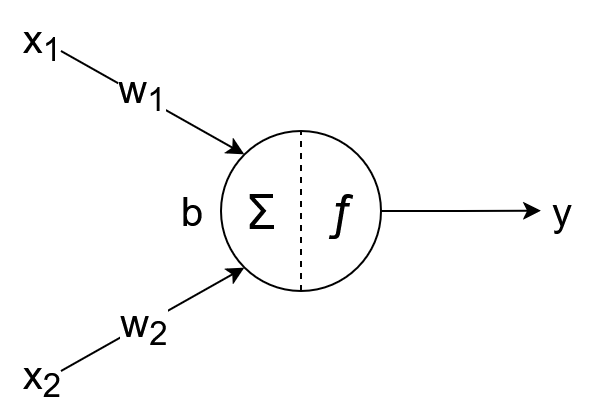
\includegraphics[width=0.7\linewidth]{images/neuron.png}
	\end{center}
	\fonte{o autor}
\end{figure}

No exemplo representado na Figura \ref{fig:neuron}, um neurônio recebe dados de entrada, $x_1$ e $x_2$, e produz uma saída $y$. Para isso, cada entrada é multiplicada por seu respectivo peso, $w_1$ e $w_2$, e somada junto a um termo de viés $b$ -- assim, a equação resultante é igual a $\sum = x_1 w_1 + x_2 w_2 + b$. Finalmente, aplica-se uma função de ativação $f$ sobre a soma para converter esse valor em um intervalo desejado -- a tangente hiperbólica produziria um número dentro do intervalo $(-1, 1)$, enquanto a sigmoide produziria um intervalo entre $(0, 1)$, por exemplo -- resultando na saída $y$ \cite{deeplearningbook}. Em outras palavras, os pesos indicam a importância, ou força, da conexão entre a entrada e o neurônio; o viés atua como um limiar de ativação que independe das entradas; e a função de ativação transforma uma entrada linear em uma saída não linear, o que permite um mapeamento complexo entre entradas e saídas. 

Uma rede neural artificial é formada pela interligação de neurônios, assim, uma camada da rede é denominada a partir de um grupo de nós interligados, que processam dados de uma maneira específica. Combinando uma camada de entrada, camadas intermediárias e uma camada de saída, obtém-se uma rede neural profunda, ilustrada na Figura \ref{fig:dnn}. Dessa forma, cada camada recebe entradas ponderadas a partir das camadas anteriores, aplicam uma função de ativação e propagam o resultado para as camadas subsequentes \cite{deeplearningbook}. Diferentes configurações destas, como a variação das conexões entre neurônios ou o emprego de funções de ativação distintas, tem por efeito especializações, ou habilidades de aprendizado específicas, assim, a utilização de múltiplas camadas permite a assimilação de representações hierárquicas complexas. \cite{reviewdeep}.

\begin{figure}[H]
	\caption{\label{fig:dnn}Representação de uma Rede Profunda}
    \begin{center}
    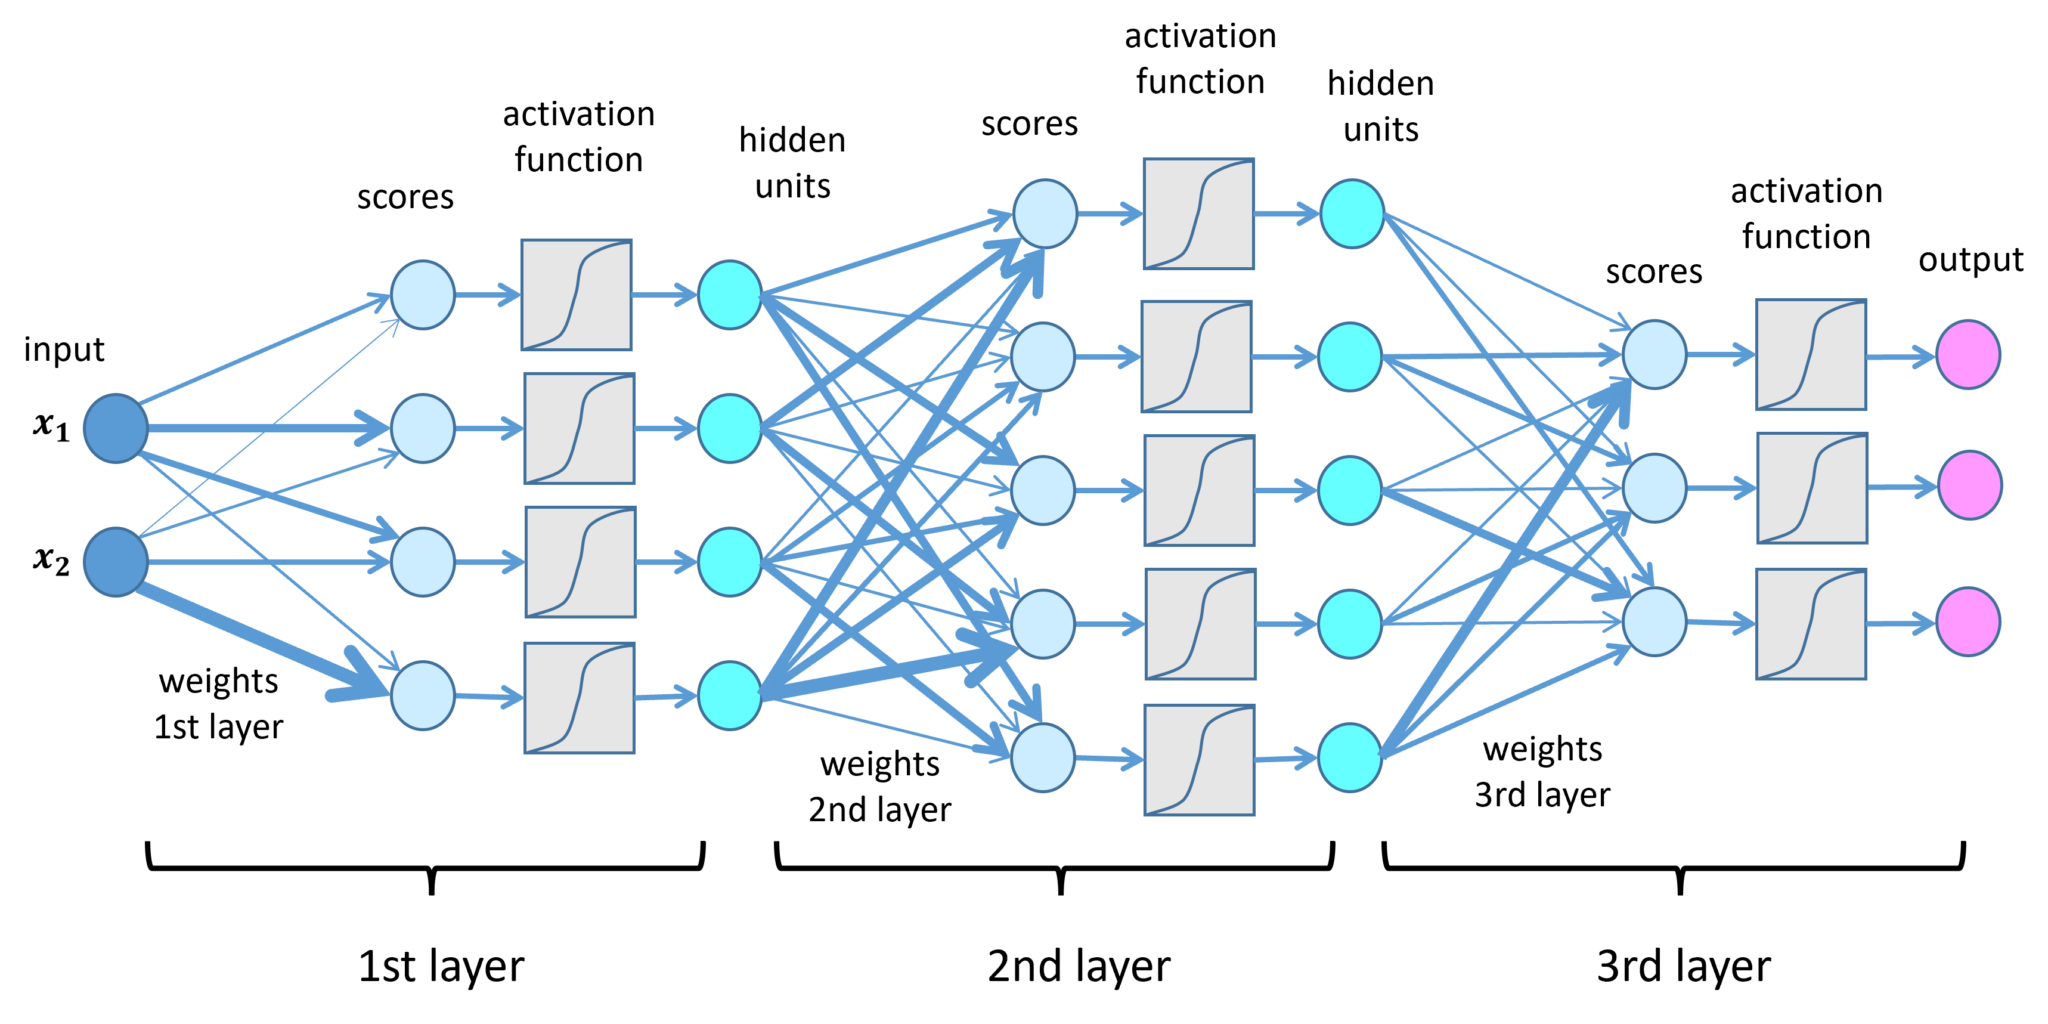
\includegraphics[width=1\linewidth]{images/dnn.png}
	\end{center}
	\fonte{\url{https://lamarr-institute.org/blog/deep-neural-networks/}. Acesso em: 25 junho 2025}
\end{figure}


O processo de aprendizado da rede é denominado treinamento e consiste na estimação e ajuste dos parâmetros através de um algoritmo de retropropagação. Seu objetivo é calcular o gradiente de uma função que mede o erro entre o valor de saída computado e o esperado, além de ajustar os pesos e vieses dos neurônios na direção oposta ao gradiente, para minimizar o erro. Esse processo é executado em cada camada, propagando o erro desde a camada de saída até a de entrada, de forma iterativa, por múltiplas épocas, até que a rede converja para uma solução otimizada \cite{deeplearningbook}, como ilustrado na Figura \ref{fig:gradientdescent}, em que o eixo $y$ representa valores de erro e o eixo $x$ valores de peso.

\begin{figure}[H]
	\caption{\label{fig:gradientdescent}Visualização do Gradiente Descendente}
    \begin{center}
    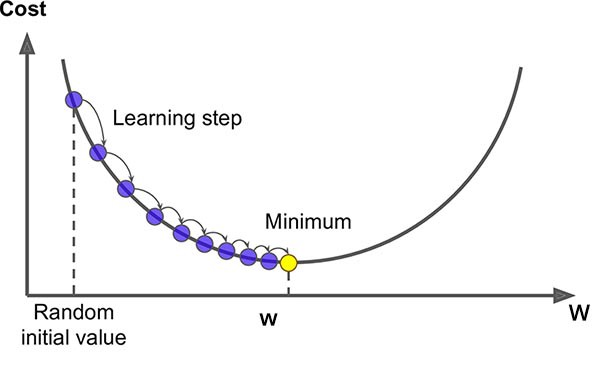
\includegraphics[width=1\linewidth]{images/gradientdescent.jpg}
	\end{center}
	\fonte{\url{https://mlpills.dev/machine-learning/gradient-descent/}. Acesso em: 25 junho 2025}
\end{figure}


\subsection{Redes Neurais Convolucionais}

Redes neurais convolucionais são tipos de redes neurais profundas especialmente úteis na área de visão computacional, especializadas na computação de dados estruturados em topologia de malha, representados matricialmente. O que propicia essa propriedade é o emprego de operações de convolução em pelo menos um módulo da rede, o que consiste em uma mudança no processamento de entrada dos neurônios: ao invés da simples soma ponderada pelos pesos, um cálculo é efetuado a partir da aplicação de um filtro sobre um \textit{input} \cite{deeplearningbook}. Dessa forma, a estrutura de um modelo básico combina camadas convolucionais com camadas de subamostragem, todas esparsamente conectadas \cite{reviewdeep}.

Convolução é uma operação matemática sobre duas funções para a criação de uma terceira, que representa, em termos simplórios, a sobreposição delas. No contexto de redes convolucionais, consiste na multiplicação de duas matrizes seguida de uma soma \cite{origindl}, como demonstrado na Figura \ref{fig:convolution}.

\begin{figure}[H]
	\caption{\label{fig:convolution}Visualização de uma Operação de Convolução}
    \begin{center}
    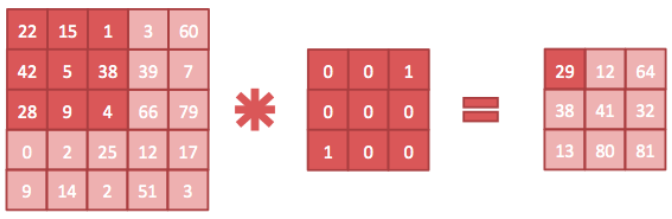
\includegraphics[width=0.75\linewidth]{images/convolution.png}
	\end{center}
	\fonte{\cite{origindl}}
\end{figure}


Um filtro -- ou \textit{kernel}, que é uma matriz de parâmetros aprendíveis -- desliza sobre os dados de entrada, a um passo definido, computando o produto escalar entre seus pesos e os valores correspondentes na região coberta, de forma a criar um mapa de características que representa a presença de padrões específicos detectados pelo filtro \cite{deeplearningbook}. Dessa forma, certas configurações, como o tamanho e os pesos do \textit{kernel}, ou o número de passos de deslizamento, controlam a resolução espacial e a capacidade de modelar relações de vizinhança, como figurativamente representado na Figura \ref{fig:nono}, em que a escolha de um filtro inicial para a detecção de bordas permite o treinamento da rede para a distinção entre gatos magros e gordos.

\begin{figure}[H]
	\caption{\label{fig:nono}Representação da Classificação de uma Imagem por uma Rede Convolucional}
    \begin{center}
    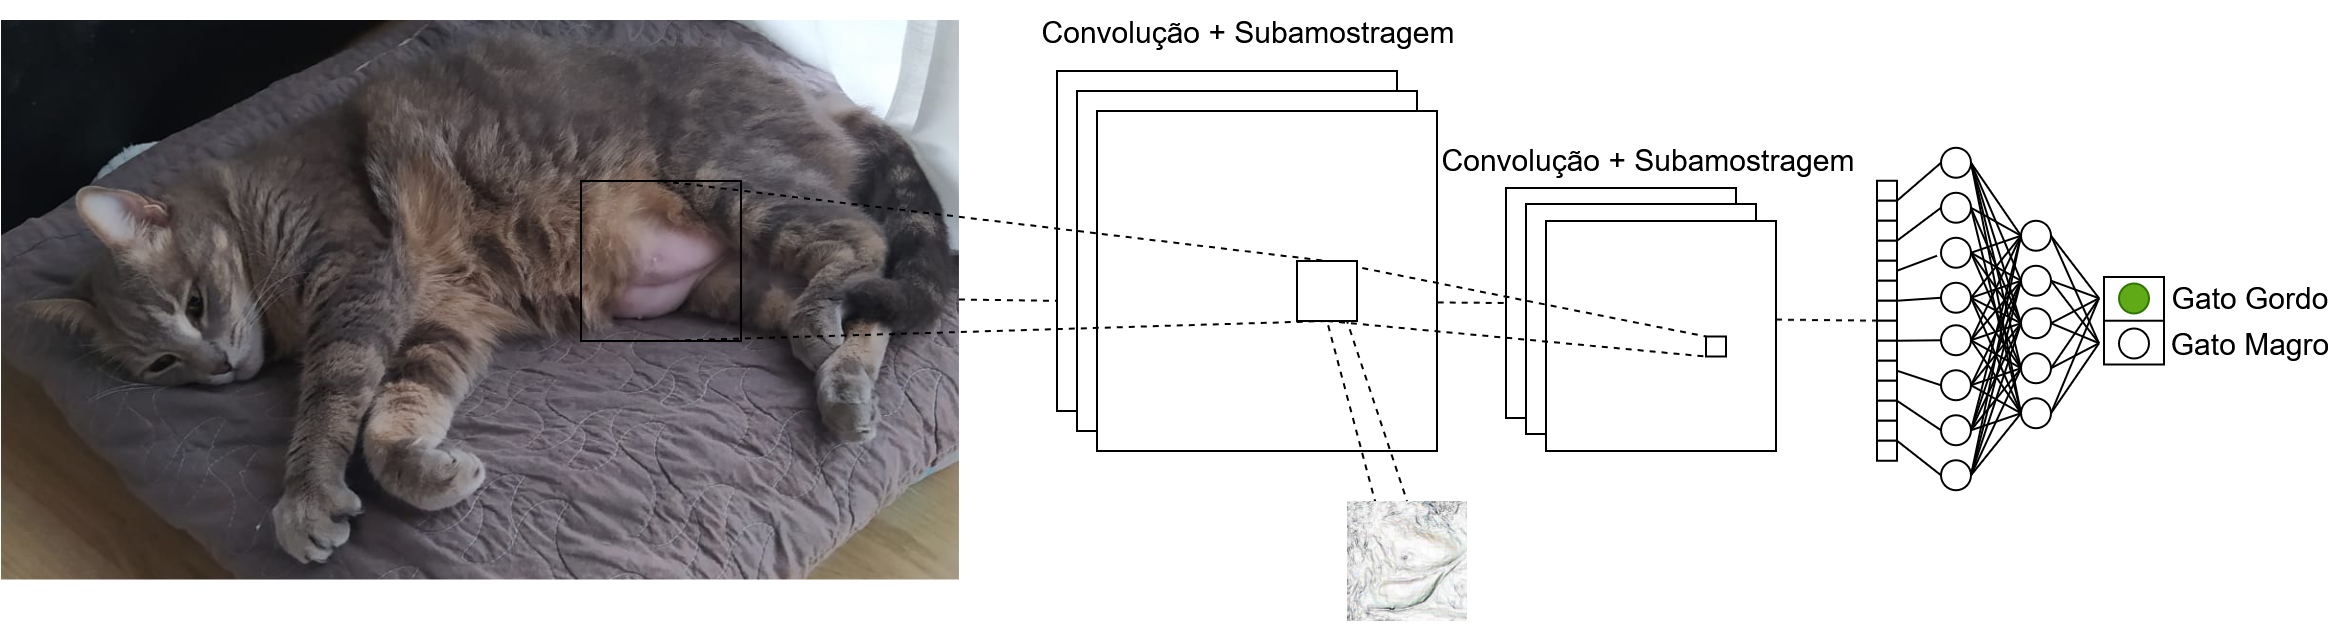
\includegraphics[width=1\linewidth]{images/nono.png}
	\end{center}
	\fonte{o autor}
\end{figure}

Outro importante aspecto das redes convolucionais são as camadas de subamostragem, que reduzem a dimensão espacial dos dados de entrada ao passo em que preservam suas características mais relevantes, processo conhecido como \textit{pooling}. Atingem isso com a obtenção de apenas uma amostra para cada região analisada, para isso, empregam estratégias como \textit{max-pooling} (extração do maior valor de entrada) e \textit{average-pooling} (extração da média dos valores de entrada). A combinação de camadas convolucionais com camadas de subamostragem conferem às essas redes três propriedades fundamentais: a invariância à pequenas transformações, distorções e translações da entrada, que permite que características sejam detectadas independentemente de sua localização; a capacidade de extrair hierarquias espaciais através da redução progressiva de dimensionalidade; e a redução do custo computacional das camadas subsequentes \cite{origindl}.

Dessa forma, a extração de \textit{features} acontece conforme a entrada percorre a rede. Utilizando como exemplo uma imagem para a entrada, as camadas iniciais capturam informações de baixo nível, como bordas, cantos e texturas. Em camadas intermediárias, essas informações passam a compor padrões semânticos locais, como delimitações de objetos, até que, em camadas mais profundas, transformam-se em caracterizações globais de alto nível, como formas completas. Isso permite que as camadas finais possam prever, ou extrair, representações complexas e abstratas \cite{reviewdeep}, como o exemplo utilizado anteriormente -- a classificação entre gatos gordos e magros.

\subsubsection{Reconhecimento Óptico de Caracteres (OCR)}

O reconhecimento óptico de caracteres (OCR), no contexto de computação, descreve um tipo de software que tem por objetivo a conversão de texto (impressos ou presentes em imagens) a um formato digital, que possa ser processável por máquina \cite{ocr}. Originalmente, os métodos de OCR baseavam-se em técnicas de segmentação da visão computacional clássica junto a heurísticas, como a segmentação de linhas e caracteres por projeções de histograma, seguida pela aplicação de regras heurísticas para identificar cada símbolo \cite{ocr2}. No entanto, as abordagens que utilizam o aprendizado de máquina -- em especial, redes convolucionais -- têm se mostrado mais eficientes e precisas \cite{ocr2}.

De acordo com \citeauthor*{ocr} \cite*{ocr}, um processo de reconhecimento de caracteres moderno tipicamente passa pelo seguinte \textit{pipeline}:

\begin{enumerate}
	\item Aquisição da imagem: obtém-se a imagem com o texto a partir de uma fonte externa, como \textit{scanner} ou câmera;
	\item Pré-processamento: aplicam-se técnicas como remoção de ruído, operações morfológicas e limiarização para melhorar a qualidade da imagem;
	\item Segmentação de caracteres: separam-se os caracteres através da análise de componentes conectados, perfis de projeção ou métodos avançados para tratar textos sobrepostos ou fragmentados;
	\item Extração de \textit{features} e classificação de caracteres: com os caracteres separados, utiliza-se uma rede convolucional para a extração e classificação de seus padrões;
	\item Pós-processamento: para refinar os resultados e aumentar a acurácia, combinam-se técnicas de processamento de linguagem natural, como corretores ortográficos e dicionários com modelos probabilísticos, como cadeias de Markov e N-gramas.
\end{enumerate}

\subsection{Processamento de Linguagem Natural}

O processamento de linguagem natural é um subcampo da inteligência artificial que se dedica ao desenvolvimento de algoritmos capazes de compreender, interpretar e processar linguagem humana de forma computacional. Tradicionalmente, as abordagens baseavam-se em métodos estatísticos, modelos de N-gramas, campos aleatórios condicionais e máquinas de vetores de suporte. Contudo, as últimas décadas têm visto a adoção de técnicas baseadas em redes neurais profundas, que demonstraram capacidade superior de capturar relações complexas entre palavras e compreender contextos linguísticos mais amplos \cite{nlp}.

Fundamentalmente, as técnicas modernas de processamento de linguagem consistem na transformação de texto em representações numéricas que preservam informações sintáticas e semânticas. \textit{Embeddings} de palavras constituem o passo base dessa transformação, que consiste em um mapeamento destas para vetores densos, onde termos semanticamente similares ocupam posições próximas \cite{nlp}. Isso possibilita o aprendizado de estruturas gramaticais e padrões linguísticos, que por sua vez permitem a predição de palavras com base em contextos previamente vistos.

As abordagens modernas de processamento de linguagem dividem-se, majoritariamente, em duas arquiteturas de redes profundas: especializações de redes neurais recorrentes, como LSTM (\textit{long short-term memory}), desenvolvidas para capturar dependências de longo prazo em sequências; ou arquiteturas \textit{Transformers}, capazes do processamento de sequências de forma paralela \cite{nlp2}.

Diferentemente dos modelos de rede apresentados anteriormente, em que os nós processam entradas de maneira independente e passam o resultado adiante, as redes neurais recorrentes utilizam conexões recorrentes, isto é, a saída de um neurônio é retroalimentada à sua camada no próximo passo de processamento, como ilustrado na Figura \ref{fig:rnn}. Essa retroalimentação permite a conservação de um estado oculto que pode ser atualizado a cada passo temporal. Isso permite a captura de padrões e relações temporais dentro de uma sequência, tornando-as boas candidatas ao processamento de texto e outros dados onde a ordem dos elementos é importante \cite{rnn}. 

\begin{figure}[H]
	\caption{\label{fig:rnn}Representação de uma Rede Neural Recorrente}
    \begin{center}
    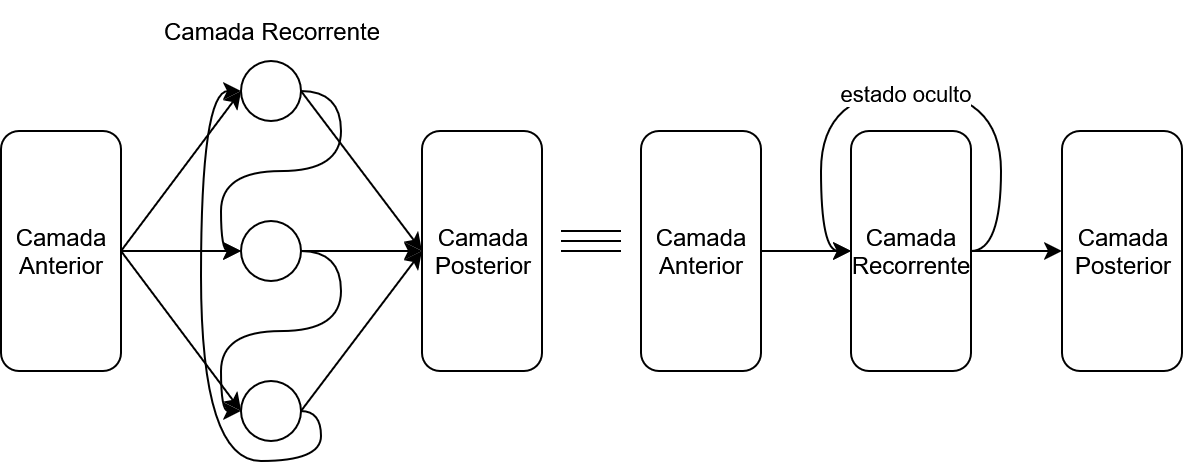
\includegraphics[width=1\linewidth]{images/rnn.png}
	\end{center}
	\fonte{o autor}
\end{figure}

Em teoria, essas redes são capazes de capturar dependências de longo prazo, no entanto, modelos básicos acabam gradualmente perdendo informações distantes conforme as sequências de entrada ficam longas \cite{nlp}. Isso ocorre por conta do problema de dissipação de gradiente, fenômeno inerente a redes profundas treinadas por \textit{backpropagation}, onde os gradientes utilizados para atualizar os pesos das camadas anteriores diminuem exponencialmente à medida que se retropropagam \cite{deeplearningbook}. Isso significa que as camadas iniciais recebem gradientes muito pequenos, o que resulta em uma atualização insignificante dos pesos e, consequentemente, aprendizado lento ou até mesmo nulo.

Para resolver essa limitação, as redes LSTM utilizam células que controlam seletivamente o fluxo de informações. Essas estruturas guardam um estado por intervalos de tempo e são compostas, de forma geral, por três mecanismos principais: \textit{forget gates} determinam quais informações devem ser descartadas; \textit{input gates} determinam quais novas informações serão armazenadas no estado da célula; \textit{output gates} determinam quais partes do estado interno influenciarão a saída. Essas decisões são tomadas a partir do cálculo de funções -- tipicamente sigmoide, que resulta em um intervalo entre 0 e 1 -- sobre parâmetros aprendíveis \cite{lstm}. Dessa forma, a rede passa a aprender a lembrar dependências de longo prazo, ou esquecer informações contextuais desnecessárias.

Embora os modelos LSTM sejam eficazes no processamento de texto, possuem uma limitação principal: precisam processar a entrada sequência a sequência -- ou palavra a palavra --, porque a computação dos estados seguintes dependem da computação dos estados anteriores. Isso faz com que o treinamento e a inferência sejam muito lentos e pouco escaláveis \cite{nlp2}.

As arquiteturas \textit{Transformer} superam essa limitação através do processamento paralelo de todos os termos da sequência de entrada. Isso é possibilitado pelas camadas de atenção, que calculam pesos que interconectam diferentes posições do \textit{input}, permitindo que o modelo foque nas palavras mais relevantes às que estão em processamento. Esse processo acontece da seguinte forma: nas camadas iniciais da rede, a sequência de \textit{embeddings} passa por três projeções lineares independentes, de forma a criar, para cada termo, vetores de consultas, chaves e valores; as camadas de atenção então computam similaridades entre as coleções de consulta e de chaves, normalizam esses escores em coeficientes para a obtenção de uma matriz de pesos, e combinam coleções de valores correspondentes de forma ponderada por esses pesos. Assim, operações aplicadas sobre consultas e chaves resultam na obtenção de valores que capturam, em cada posição, as dependências contextuais mais relevantes de toda a sequência -- tudo isso de modo paralelo \cite{transformer}.

Dessa forma, os modelos \textit{Transformer} estruturam-se em duas partes, a primeira consiste na utilização de blocos de codificação, que aplicam sucessivamente camadas de atenção e de propagação comum, assim, esses blocos "prestam atenção" somente na sequência de entrada. A segunda emprega blocos de decodificação que, em relação aos blocos de codificação, adicionam camadas intermediárias de atenção codificador-decodificador. Essas camadas recebem em sua entrada, além da saída das camadas de atenção anteriores, as saídas diretas dos blocos de codificação e, dessa forma, "prestam atenção" tanto na sequência de saída quanto a de entrada \cite{transformer}. A consequência dessa arquitetura é que o processo de codificação transforma as sequências de entrada em representações abstratas, que incorporam informações de todo o contexto, enquanto a decodificação utiliza essas representações para gerar novos termos de saída, condicionando cada novo elemento tanto às informações abstraídas da entrada quanto ao contexto já produzido pela própria sequência de saída \cite{transformer}.

\section{Análise Multimodal}

A análise multimodal refere-se à integração de informações provenientes de diferentes modalidades de dados, como texto, imagem, áudio e vídeo. Esse tipo de análise reconhece que informações relevantes podem estar distribuídas entre diferentes categorias de dados, sendo que cada uma contribui com aspectos únicos e complementares para a compreensão completa do conteúdo \cite{multimodalsurvey}. Utilizando o caso do presente estudo como exemplo, em um documento acadêmico, o texto isoladamente pode parecer legítimo, no entanto, quando combinado com inconsistências visuais, pode revelar sinais de falsificação, e vice-versa.

No contexto de aprendizado de máquina, o processo conhecido como fusão multimodal consiste em combinar as diferentes representações de tipos de dados em uma unificada, possibilitando que os modelos consigam aprender as características mais relevantes em diferentes domínios de forma prática e eficiente, o que resulta em representações mais ricas e discriminativas \cite{multimodalsurvey,multimodalforgery}. Dessa forma, as estratégias de fusão são normalmente classificadas em quatro categorias principais, dependendo do momento em que ocorrem: fusão precoce, onde as representações brutas são combinadas e servem de entrada para o modelo de aprendizado; fusão intermediária, onde as representações são incorporadas durante as etapas de aprendizado, como em camadas intermediárias de uma rede neural; fusão tardia, onde as decisões de classificadores de modalidades distintas são combinadas; e fusão híbrida, que combina diferentes estratégias de fusão \cite{multimodalsurvey}.

A metodologia deste trabalho utilizará a fusão precoce para combinar os dados extraídos, representados em vetores, a partir das modalidades visuais e textuais. Para isso, \citeauthor*{multimodalmeta} \cite*{multimodalmeta} e \citeauthor*{multimodalforgery} \cite*{multimodalforgery} apresentam diferentes técnicas:

\begin{itemize}
	\item Concatenação básica: abordagem mais simples e direta. Consiste na concatenação simples dos vetores de dados;
	\item Adição elemento a elemento: consiste na soma direta entre os respectivos elementos de cada modalidade;
	\item Transformação bilinear: consiste no produto matricial entre os vetores;
	\item Soma ponderada (\textit{gated summation}): utiliza uma rede neural com funções de ativação específicas, como \textit{weighted sigmoid gate units}, para somar os elementos de forma ponderada, como se o modelo passasse a entender a importância de cada fonte de informação;
	\item Produto ponderado: semelhante à soma ponderada utiliza uma rede neural, mas emprega mecanismos de atenção para o aprendizado, dessa forma, o resultado é o produto matricial entre os vetores, ponderado por uma matriz de pesos.
\end{itemize}

Não existe uma técnica ótima para todos os casos, visto que são subjetivas às características específicas dos domínios ao qual se deseja a união e, assim, a escolha pela melhor abordagem é geralmente determinada pela análise empírica dos resultados \cite{multimodalmeta}.

Além disso, o emprego da fusão multimodal é geralmente associado a outras estratégias auxiliares, que podem tratar tanto os vetores de representação antes da fusão quanto o resultante. Por exemplo, diferentes modalidades possuem características estatísticas e distribuições distintas, dessa forma, pode ser necessário pré-processamento para normalização das escalas dos dados. Da mesma forma, o vetor resultante, por juntar dados muitas vezes situados em espaços de alta dimensionalidade, precisa da aplicação de técnicas de redução dimensional para evitar problemas relacionados à \textit{maldição da dimensionalidade}, termo cunhado por \citeauthor*{bellmancurse} \cite*{bellmancurse}, que explica que ao lidar com dados em espaços de alta dimensão, sua amostragem e modelagem torna-se progressivamente mais esparsa e difícil dado que o volume do espaço cresce exponencialmente.

\section{Algoritmos de Agrupamento}

No contexto de aprendizado de máquina, as técnicas de agrupamento, ou \textit{clustering}, têm por objetivo a organização de uma coleção de dados em grupos, ou \textit{clusters}, de forma que os elementos dentro de um mesmo grupo tenham muito mais similaridades entre si do que entre elementos em outros grupos. Essas técnicas geralmente são utilizadas quando não se tem conhecimento sobre como os dados podem ser categorizados, dessa forma, tradicionalmente são associadas à aprendizagem não supervisionada \cite{cluster1}. Assim, têm como propósito descobrir estruturações, relações, associações ou hierarquias ocultas dentro da coleção, de maneira a proporcionar melhor compreensão sobre os dados e seus processos subjacentes de criação \cite{cluster2}.

Como trata-se de uma larga área de estudo, os algoritmos de \textit{clustering} variam significativamente em sua compreensão do que constitui um \textit{cluster} e de como este pode ser encontrado de forma eficiente, dessa forma, noções populares incluem grupos com pequenas distâncias entre membros, áreas densas do espaço de dados, intervalos ou distribuições estatísticas específicas \cite{cluster2}. Por fins de brevidade, aqui explicam-se os métodos de agrupamento particional -- que buscam criar grupos a partir do particionamento único da coleção de dados, de forma que um elemento não pertença a mais de um grupo \cite{cluster1} --, em especial, algoritmos baseados em distância e em densidade.

Para os algoritmos baseados em distância, cada \textit{cluster} é representado por um protótipo e a atribuição de elementos a estes é guiada pela minimização de alguma medida de dissimilaridade. Em termos mais concretos, tanto os \textit{clusters} quanto os dados são tipicamente traduzidos como pontos em um espaço. Busca-se então a minimização de uma função de custo, como a soma das distâncias quadráticas entre cada elemento e um \textit{cluster}. Isso acontece através do calculo iterativo da função de custo seguido do ajuste posicional do \textit{cluster}, processo repetido alternadamente até que a valor de custo fique abaixo de um limiar determinado, garantindo a convergência do algoritmo, ou seja, a posição ótima do agrupamento \cite{cluster1, cluster2}.

\begin{figure}[H]
	\caption{\label{fig:kmeans}Representação de um Algoritmo de \textit{Clustering} por Distância}
    \begin{center}
    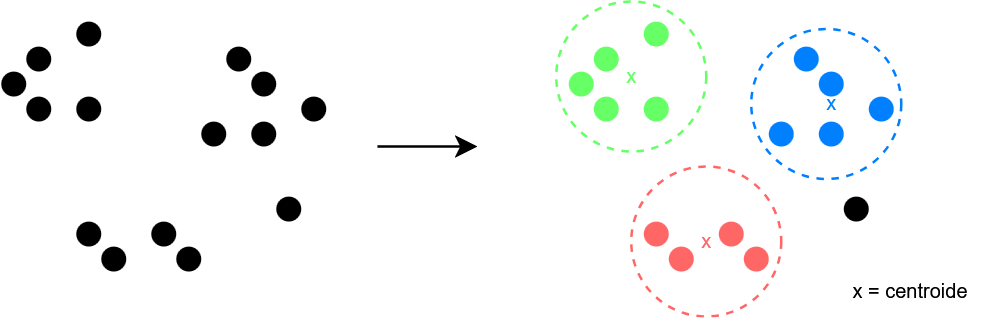
\includegraphics[width=1\linewidth]{images/kmeans.png}
	\end{center}
	\fonte{o autor}
\end{figure}

Os algoritmos baseados em densidade consideram que \textit{clusters} são regiões de alta densidade de dados separadas por áreas de baixa densidade, assim, tanto o formato dos agrupamentos quanto a distribuição dos elementos podem ser feitos de forma arbitrária. O algoritmo DBSCAN pode ser utilizado para exemplificar esse conceito: definem-se os parâmetros $\epsilon$ (raio de vizinhança) e $MinPts$ (número mínimo de pontos ou elementos), assim, um ponto considera outro como vizinho quando está dentro de $\epsilon$. Então, conta-se o número de vizinhos para cada ponto: aqueles com vizinhança densa -- isto é, número de vizinhos maior que $MinPts$ -- tornam-se pontos centrais e formam núcleos de \textit{clusters}; aqueles atingíveis por vizinhança dentro de um \textit{cluster} são absorvidos e chamados de pontos de fronteira; e aqueles pouco densos e não atingíveis são classificados como ruído. \cite{cluster1}.

\begin{figure}[H]
	\caption{\label{fig:dbscan}Representação do Algoritmo DBSCAN}
    \begin{center}
    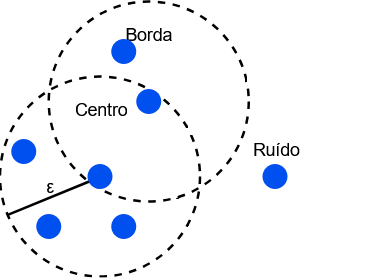
\includegraphics[width=.5\linewidth]{images/dbscan.png}
	\end{center}
	\fonte{o autor}
\end{figure}

\subsection{Detecção de Anomalias}

A detecção de anomalias é definida como o processo de identificar padrões em um conjunto de dados cujo comportamento difere significativamente do esperado, assim, pode ser tratado como um problema de identificação de \textit{outliers} ou ruídos em algoritmos de agrupamento. Quando identificadas, embora nem sempre representem atividades maliciosas, frequentemente indicam eventos de interesse que merecem investigação \cite{anomaly, cluster2}.

A metodologia típica segue três etapas principais: parametrização e pré-processamento, onde os dados são normalizados em formatos comuns; treinamento, onde são construídos modelos de comportamento normal; e finalmente, detecção, em que uma nova observação é comparada aos modelos construídos \cite{anomaly}. Dessa forma, a detecção de anomalias baseada em \textit{clustering} funciona estabelecendo modelos de normalidade através do agrupamento de dados e, posteriormente identificando novos elementos que apresentam desvios expressivos desses modelos de referência.